% Name: Shortest path
% Description: Dijkstra's result from A to F: the path in orange and each vertex's distance beside it.
% Tags: shortest path, Dijkstra, weighted graph, algorithm

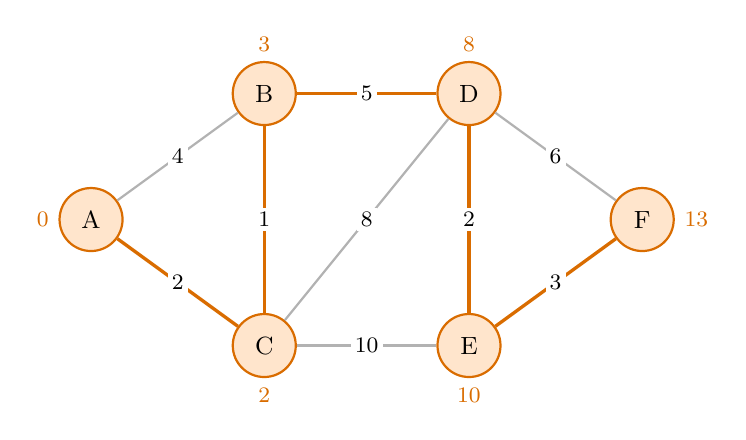
\begin{tikzpicture}[
  vertex/.style={circle, draw, thick, fill=white, minimum size=8mm, font=\small},
  onpath/.style={vertex, fill=orange!20, draw=orange!85!black},
  dist/.style={font=\footnotesize, text=orange!85!black},
  weight/.style={font=\footnotesize, fill=white, inner sep=1.5pt},
]
  \node[onpath, label={[dist]left:0}] (A) at (0,0) {A};
  \node[onpath, label={[dist]above:3}] (B) at (2.2,1.6) {B};
  \node[onpath, label={[dist]below:2}] (C) at (2.2,-1.6) {C};
  \node[onpath, label={[dist]above:8}] (D) at (4.8,1.6) {D};
  \node[onpath, label={[dist]below:10}] (E) at (4.8,-1.6) {E};
  \node[onpath, label={[dist]right:13}] (F) at (7,0) {F};

  \foreach \u/\v in {A/B, C/D, C/E, D/F}
    \draw[thick, gray!60] (\u) -- (\v);
  \foreach \u/\v in {A/C, C/B, B/D, D/E, E/F}
    \draw[very thick, orange!85!black] (\u) -- (\v);
  \foreach \u/\v/\w in {A/B/4, A/C/2, B/C/1, B/D/5, C/D/8, C/E/10, D/E/2, D/F/6, E/F/3}
    \path (\u) -- node[weight] {\w} (\v);
\end{tikzpicture}
